\documentclass[11pt]{article}
\usepackage[margin=1in]{geometry}
\usepackage{amsmath,amssymb,amsfonts,bm,mathtools}
\usepackage{booktabs}
\usepackage{tikz}
\usetikzlibrary{arrows.meta,positioning,shapes.geometric}
\usepackage{hyperref}

\title{PhILR-VAE: A Rigorous Mathematical Specification}
\author{biomeVAE documentation}
\date{}

\begin{document}
\maketitle

\section{Setup and notation}
Let $x\in\mathbb{N}_0^p$ denote observed counts over $p$ taxa, with library size
\begin{equation}
N=\sum_{i=1}^p x_i.
\end{equation}
Given pseudocount $\alpha>0$, define the closed composition
\begin{equation}
c_i=\frac{x_i+\alpha}{\sum_{j=1}^p (x_j+\alpha)},
\qquad c\in\Delta^{p-1}:=\{u\in\mathbb{R}_{>0}^p:\sum_i u_i=1\}.
\end{equation}

\section{PhILR basis and transform}
A taxonomy tree induces a sequential binary partition (SBP). For each split $(R,S)$, $R\cap S=\emptyset$, $|R|=r$, $|S|=s$, define contrast entries
\begin{equation}
\psi_i=
\begin{cases}
\sqrt{\dfrac{s}{r(r+s)}} & i\in R,\\[4pt]
-\sqrt{\dfrac{r}{s(r+s)}} & i\in S,\\[4pt]
0 & \text{otherwise}.
\end{cases}
\end{equation}
Stacking all $p-1$ contrasts gives $\Psi\in\mathbb{R}^{p\times(p-1)}$ with orthonormal columns in $\mathbf{1}^\perp$.

\paragraph{Forward map.}
\begin{equation}
y=\operatorname{ilr}(c)=\log(c)^\top\Psi\in\mathbb{R}^{p-1}.
\end{equation}

\paragraph{Inverse map.}
\begin{equation}
\tilde\ell = y\Psi^\top\in\mathbb{R}^p,
\qquad
\hat c_i=\frac{\exp(\tilde\ell_i)}{\sum_j \exp(\tilde\ell_j)}.
\end{equation}

\paragraph{Isometry.}
For compositions $c^{(1)},c^{(2)}$ and ilr coordinates $y^{(k)}$, one has
\begin{equation}
\|y^{(1)}-y^{(2)}\|_2 = d_A\left(c^{(1)},c^{(2)}\right),
\end{equation}
where $d_A$ is Aitchison distance.

\section{Variational model}
Prior and variational posterior:
\begin{equation}
p(z)=\mathcal{N}(0,I_d),
\qquad
q_\phi(z\mid x)=\mathcal{N}\big(\mu_\phi(x),\operatorname{diag}(\sigma_\phi^2(x))\big).
\end{equation}
Reparameterization:
\begin{equation}
z=\mu_\phi(x)+\sigma_\phi(x)\odot \varepsilon,
\qquad \varepsilon\sim\mathcal{N}(0,I_d).
\end{equation}
Decoder produces $\hat y=g_\theta(z)$, then
\begin{equation}
\hat c=\operatorname{ilr}^{-1}(\hat y),
\qquad
\hat\mu = N\hat c.
\end{equation}

\section{Negative Binomial likelihood}
Each feature follows
\begin{equation}
x_i\sim\operatorname{NB}(\mu_i,\theta_i),\qquad \theta_i>0,
\end{equation}
with mean--variance relation
\begin{equation}
\operatorname{Var}(x_i)=\mu_i+\frac{\mu_i^2}{\theta_i}.
\end{equation}
Log-likelihood term:
\begin{equation}
\log p(x_i\mid\mu_i,\theta_i)
= \log\Gamma(x_i+\theta_i)-\log\Gamma(\theta_i)-\log\Gamma(x_i+1)
+\theta_i\log\frac{\theta_i}{\theta_i+\mu_i}
+x_i\log\frac{\mu_i}{\theta_i+\mu_i}.
\end{equation}

\section{Objective and KL warmup}
Training minimizes
\begin{equation}
\mathcal{L}
= -\mathbb{E}_{q_\phi(z\mid x)}[\log p_\theta(x\mid z)]
+\beta_t\,\mathrm{KL}\left(q_\phi(z\mid x)\Vert p(z)\right).
\end{equation}
For diagonal Gaussians,
\begin{equation}
\mathrm{KL}
=\frac12\sum_{j=1}^d\left(\mu_j^2+\sigma_j^2-1-\log\sigma_j^2\right).
\end{equation}
With warmup length $T$ and $\beta_{\max}$,
\begin{equation}
\beta_t=\min\left(\beta_{\max},\beta_{\max}\frac{t}{T}\right).
\end{equation}

\section{Diagram: computational graph}
\begin{center}
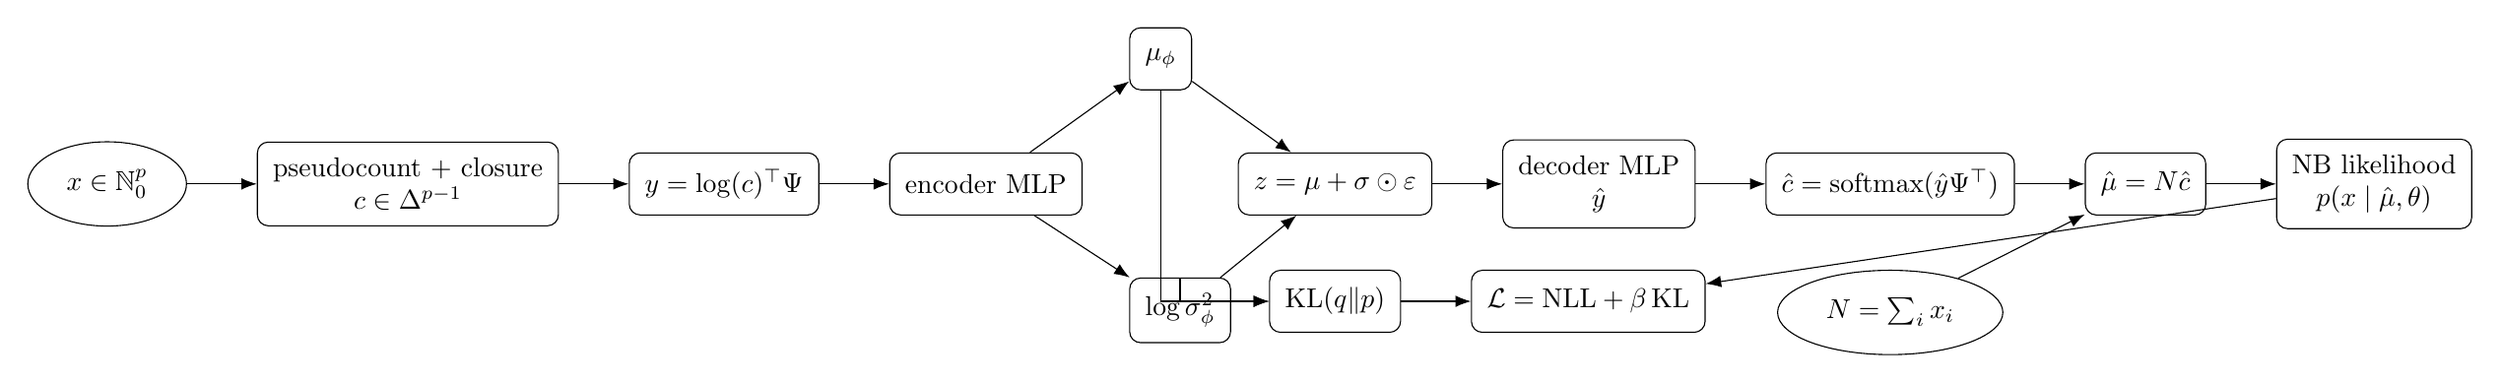
\begin{tikzpicture}[
  node distance=7mm and 9mm,
  block/.style={rectangle,rounded corners,draw,align=center,minimum height=8mm,inner sep=2mm},
  io/.style={ellipse,draw,align=center,minimum height=8mm,inner sep=2mm},
  >={Latex[length=2mm]}
]
\node[io] (x) {$x\in\mathbb{N}_0^p$};
\node[block,right=of x] (close) {pseudocount + closure\\$c\in\Delta^{p-1}$};
\node[block,right=of close] (philr) {$y=\log(c)^\top\Psi$};
\node[block,right=of philr] (enc) {encoder MLP};
\node[block,above right=8mm and 6mm of enc] (mu) {$\mu_\phi$};
\node[block,below right=8mm and 6mm of enc] (lv) {$\log\sigma_\phi^2$};
\node[block,right=20mm of enc] (z) {$z=\mu+\sigma\odot\varepsilon$};
\node[block,right=of z] (dec) {decoder MLP\\$\hat y$};
\node[block,right=of dec] (inv) {$\hat c=\mathrm{softmax}(\hat y\Psi^\top)$};
\node[io,below=of inv] (N) {$N=\sum_i x_i$};
\node[block,right=of inv] (muhat) {$\hat\mu=N\hat c$};
\node[block,right=of muhat] (nb) {NB likelihood\\$p(x\mid\hat\mu,\theta)$};
\node[block,below=of z] (kl) {$\mathrm{KL}(q\Vert p)$};
\node[block,right=of kl] (loss) {$\mathcal L = \mathrm{NLL}+\beta\,\mathrm{KL}$};

\draw[->] (x) -- (close);
\draw[->] (close) -- (philr);
\draw[->] (philr) -- (enc);
\draw[->] (enc) -- (mu);
\draw[->] (enc) -- (lv);
\draw[->] (mu) -- (z);
\draw[->] (lv) -- (z);
\draw[->] (z) -- (dec);
\draw[->] (dec) -- (inv);
\draw[->] (inv) -- (muhat);
\draw[->] (N) -- (muhat);
\draw[->] (muhat) -- (nb);
\draw[->] (mu) |- (kl);
\draw[->] (lv) |- (kl);
\draw[->] (nb) -- (loss);
\draw[->] (kl) -- (loss);
\end{tikzpicture}
\end{center}

\section{Key modeling consequences}
\begin{itemize}
\item Compositional constraints are exact (simplex by construction).
\item Tree structure is encoded in $\Psi$ (taxonomy-aware balances).
\item Euclidean distance in ilr coordinates is Aitchison-correct.
\item Library size is handled analytically ($\hat\mu=N\hat c$), improving identifiability between composition and depth.
\item NB likelihood handles overdispersion in count data.
\end{itemize}

\end{document}
